%\documentclass[handout]{beamer}
\documentclass{beamer}

\usepackage{beamerthemesplit}
\usepackage{shadowtext}
\usepackage{color}
\usepackage{xcolor}
\usepackage[utf8]{inputenc}

 \usetheme[]{Madrid}
%\usetheme[]{Copenhagen}
%\usetheme{Warsaw}

% El que uso habitualmente:
%\usetheme[height=0.7cm]{Rochester}

% A dark look
%\usecolortheme{beetle}
% A light look:
 \usecolortheme{dolphin}
 
\setbeamertemplate{footline}
{
  \leavevmode%
  \hbox{%
  \begin{beamercolorbox}[wd=.5\paperwidth,ht=2.25ex,dp=1ex,center]{author in head/foot}%
    \usebeamerfont{author in head/foot}\insertshortauthor
  \end{beamercolorbox}%
  \begin{beamercolorbox}[wd=.5\paperwidth,ht=2.25ex,dp=1ex,center]{title in head/foot}%
    \usebeamerfont{title in head/foot}\insertshorttitle\hspace*{3em}
    \insertframenumber{} / \inserttotalframenumber\hspace*{1ex}
  \end{beamercolorbox}}%
  \vskip0pt%
}
\makeatletter

\setbeamertemplate{navigation symbols}{} 

%\usepackage{wrapfig}
\setbeamercovered{transparent}

\usepackage{geometry}
%\geometry{landscape}
\usepackage{multimedia}

\usepackage{bm}%bold matH

%\usepackage{shade}
\usepackage{fancybox}
 
\usepackage{amssymb}

%\documentclass[handout]{beamer}
\documentclass{beamer}

\usepackage{beamerthemesplit}
\usepackage{shadowtext}
\usepackage{color}
\usepackage{xcolor}
\usepackage[utf8]{inputenc}

 \usetheme[]{Madrid}
%\usetheme[]{Copenhagen}
%\usetheme{Warsaw}

% El que uso habitualmente:
%\usetheme[height=0.7cm]{Rochester}

% A dark look
%\usecolortheme{beetle}
% A light look:
 \usecolortheme{dolphin}
 
\setbeamertemplate{footline}
{
  \leavevmode%
  \hbox{%
  \begin{beamercolorbox}[wd=.5\paperwidth,ht=2.25ex,dp=1ex,center]{author in head/foot}%
    \usebeamerfont{author in head/foot}\insertshortauthor
  \end{beamercolorbox}%
  \begin{beamercolorbox}[wd=.5\paperwidth,ht=2.25ex,dp=1ex,center]{title in head/foot}%
    \usebeamerfont{title in head/foot}\insertshorttitle\hspace*{3em}
    \insertframenumber{} / \inserttotalframenumber\hspace*{1ex}
  \end{beamercolorbox}}%
  \vskip0pt%
}
\makeatletter

\setbeamertemplate{navigation symbols}{} 

%\usepackage{wrapfig}
\setbeamercovered{transparent}

\usepackage{geometry}
%\geometry{landscape}
\usepackage{multimedia}

\usepackage{bm}%bold matH

%\usepackage{shade}
\usepackage{fancybox}
 
\usepackage{amssymb}

%\documentclass[handout]{beamer}
\documentclass{beamer}

\usepackage{beamerthemesplit}
\usepackage{shadowtext}
\usepackage{color}
\usepackage{xcolor}
\usepackage[utf8]{inputenc}

 \usetheme[]{Madrid}
%\usetheme[]{Copenhagen}
%\usetheme{Warsaw}

% El que uso habitualmente:
%\usetheme[height=0.7cm]{Rochester}

% A dark look
%\usecolortheme{beetle}
% A light look:
 \usecolortheme{dolphin}
 
\setbeamertemplate{footline}
{
  \leavevmode%
  \hbox{%
  \begin{beamercolorbox}[wd=.5\paperwidth,ht=2.25ex,dp=1ex,center]{author in head/foot}%
    \usebeamerfont{author in head/foot}\insertshortauthor
  \end{beamercolorbox}%
  \begin{beamercolorbox}[wd=.5\paperwidth,ht=2.25ex,dp=1ex,center]{title in head/foot}%
    \usebeamerfont{title in head/foot}\insertshorttitle\hspace*{3em}
    \insertframenumber{} / \inserttotalframenumber\hspace*{1ex}
  \end{beamercolorbox}}%
  \vskip0pt%
}
\makeatletter

\setbeamertemplate{navigation symbols}{} 

%\usepackage{wrapfig}
\setbeamercovered{transparent}

\usepackage{geometry}
%\geometry{landscape}
\usepackage{multimedia}

\usepackage{bm}%bold matH

%\usepackage{shade}
\usepackage{fancybox}
 
\usepackage{amssymb}

%\documentclass[handout]{beamer}
\documentclass{beamer}

\usepackage{beamerthemesplit}
\usepackage{shadowtext}
\usepackage{color}
\usepackage{xcolor}
\usepackage[utf8]{inputenc}

 \usetheme[]{Madrid}
%\usetheme[]{Copenhagen}
%\usetheme{Warsaw}

% El que uso habitualmente:
%\usetheme[height=0.7cm]{Rochester}

% A dark look
%\usecolortheme{beetle}
% A light look:
 \usecolortheme{dolphin}
 
\setbeamertemplate{footline}
{
  \leavevmode%
  \hbox{%
  \begin{beamercolorbox}[wd=.5\paperwidth,ht=2.25ex,dp=1ex,center]{author in head/foot}%
    \usebeamerfont{author in head/foot}\insertshortauthor
  \end{beamercolorbox}%
  \begin{beamercolorbox}[wd=.5\paperwidth,ht=2.25ex,dp=1ex,center]{title in head/foot}%
    \usebeamerfont{title in head/foot}\insertshorttitle\hspace*{3em}
    \insertframenumber{} / \inserttotalframenumber\hspace*{1ex}
  \end{beamercolorbox}}%
  \vskip0pt%
}
\makeatletter

\setbeamertemplate{navigation symbols}{} 

%\usepackage{wrapfig}
\setbeamercovered{transparent}

\usepackage{geometry}
%\geometry{landscape}
\usepackage{multimedia}

\usepackage{bm}%bold matH

%\usepackage{shade}
\usepackage{fancybox}
 
\usepackage{amssymb}

\input{talk.macros}

\title[Tomography: UCoMP versus AIA versus KCOR]
{\bf Tomography: UCoMP versus AIA versus KCOR}
\author[Vasquez \& Nuevo]
       {
       {\bf 
       Alberto M. Vasquez \& Federico A. Nuevo}
       \vskip 0.25cm
       {\bf 
\tiny
Instituto de Astronomía y Física del Espacio (IAFE), Buenos Aires--Argentina\\
       }
       }
\institute[]
{
\begin{center}
\framebox{\includegraphics[height=0.125\linewidth]{fig/logo_IAFE.eps}}
\vskip 3cm
{\bf March 2025}
\end{center}
}

\begin{document}


\frame{
\titulo{Tomography: UCoMP versus AIA versus KCOR}
{\tiny\sf
\begin{itemize}
\item \azul{Solar rotational tomography (SRT)} makes use of 1/2 solar rotation (14-day) long sequences of coronal images to determine the \azul{3D distribution of various physical quantities} of the corona, depending on the observed wavelength range.
\salto
\item Using \azul{WL pB} images (e.g. KCOR, C2, Metis), SRT allows determination of the \azul{3D $\Ne$}.
\salto
\item Using \azul{EUV} images with a given filter (e.g. AIA 171\,\AA), SRT allows determination of the \azul{3D band-emissivity}.\\ 
Based on the reconstructed band-emissivity for various filters independently (e.g. AIA 171, 193, and 211\,\AA),\\ 
a local-DEM analysis can be carried out at each location of the corona to determine the \azul{3D $\Ne$} and \azul{$\Te$}.\\ 
The combined procedure is known as DEM-Tomography, or \azul{DEMT}.
\salto
\item Using \azul{UCoMP} total-line (wavelength-integrated) images, SRT allows determination of the \azul{3D line emissivity}.
\salto 
\item For a specific period (September 2022), we carried out:
\saltito
a) \azul{UCoMP-SRT} with 1074 and 1079 nm images to determine their respective \azul{3D emissivity maps}.\\
\ \ \ \ The 1074:1079 emissivity-ratio can then be used to determine 3D $\Ne$.
\saltito
b) \azul{AIA-DEMT} (using filters 171, 193 and 211\,\AA) to determine the \azul{3D $\Ne$} and \azul{$\Te$},\\
\ \ \ \ in turn used with CHIANTI to compute \azul{3D synthetic emissivity maps} for the lines at 1074 and 1079 nm.
\saltito
c) \azul{KCOR-SRT} to determine the 3D distribution of $\Ne$.
\salto
\item These instruments allow reconstructions over a common range of heights $1.1-1.2\,\Rs$. We compare:
\saltito 
1) The tomographic UCoMP-SRT line emissivities against the synthetic prediction based on AIA-DEMT.
\saltito
2) {The 3D $\Ne$ derived from UCoMP-SRT, derived from AIA-DEMT, and derived from KCOR-SRT.}
\end{itemize}
}}

\frame{
\titulo{3D Coronal Emissivity at 1074 nm}
{\footnotesize\sf
\begin{center}
Lat/Lon maps of UCoMP 3D \azul{Tomographic} 1074-Emissivity\\
\includegraphics[width=0.32\textwidth,clip=]{fig/x_comp1074_1_105_Rsun.jpg}
\includegraphics[width=0.32\textwidth,clip=]{fig/x_comp1074_1_145_Rsun.jpg}
\includegraphics[width=0.32\textwidth,clip=]{fig/x_comp1074_1_195_Rsun.jpg}
\salto
Lat/Lon maps of AIA(171-193-211)-DEMT 3D \azul{Synthetic} 1074-Emissivity\\
\includegraphics[width=0.32\textwidth,clip=]{fig/x_comp1074_synth_1_105_Rsun.jpg}
\includegraphics[width=0.32\textwidth,clip=]{fig/x_comp1074_synth_1_145_Rsun.jpg}
\includegraphics[width=0.32\textwidth,clip=]{fig/x_comp1074_synth_1_195_Rsun.jpg}
\salto
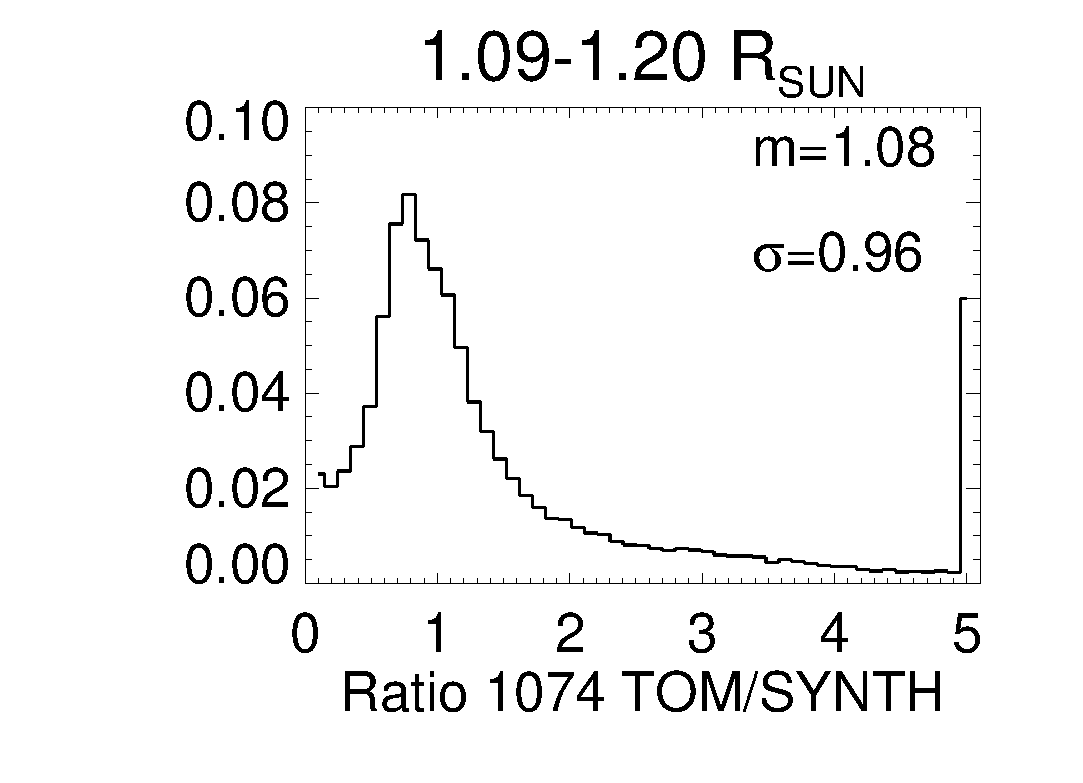
\includegraphics[height=0.2\textwidth,clip=]{fig/comparison_ucomp_Sept2022_tom_vs_synth_E1074_ratio_range1_090-1_200_Rsun.eps}
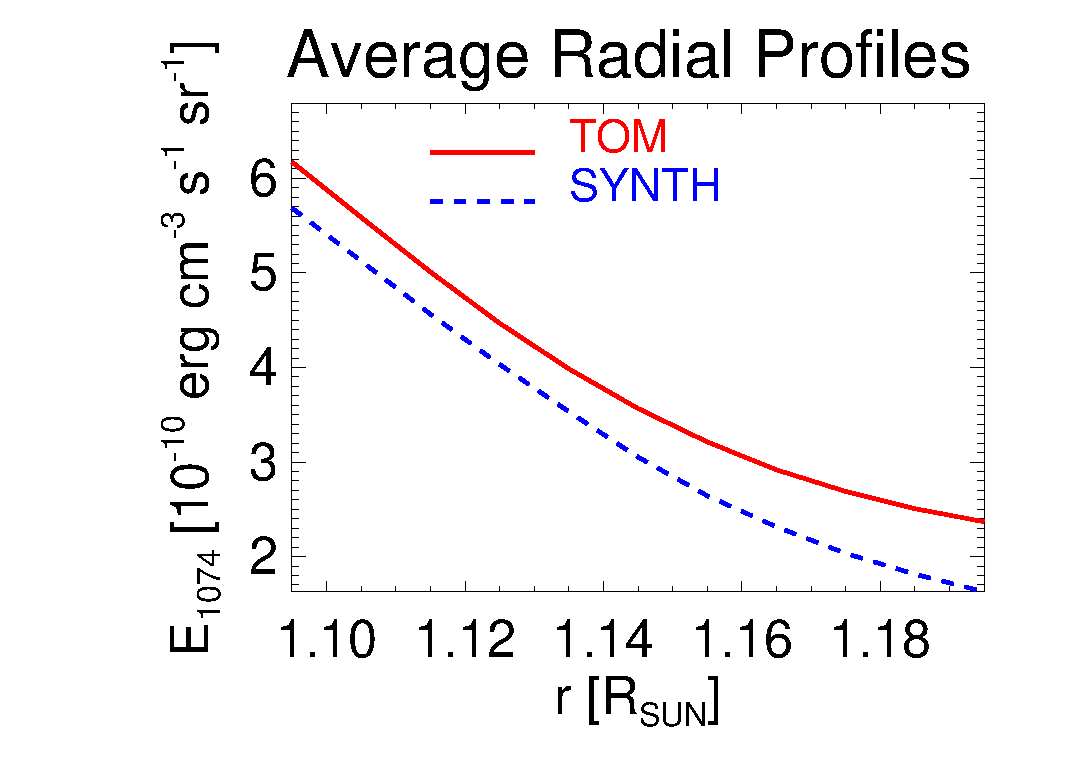
\includegraphics[height=0.2\textwidth,clip=]{fig/Average_Radial_Profiles_ucomp_Sept2022_tom_vs_synth_E1074.eps}
\end{center}
}
}

\frame{
\titulo{3D Coronal Emissivity at 1079 nm}
{\footnotesize\sf
\begin{center}
Lat/Lon maps of UCoMP 3D \azul{Tomographic} 1079-Emissivity\\
\includegraphics[width=0.32\textwidth,clip=]{fig/x_comp1079_1_105_Rsun.jpg}
\includegraphics[width=0.32\textwidth,clip=]{fig/x_comp1079_1_145_Rsun.jpg}
\includegraphics[width=0.32\textwidth,clip=]{fig/x_comp1079_1_195_Rsun.jpg}
\salto
Lat/Lon maps of AIA(171-193-211)-DEMT 3D \azul{Synthetic} 1079-Emissivity\\
\includegraphics[width=0.32\textwidth,clip=]{fig/x_comp1079_synth_1_105_Rsun.jpg}
\includegraphics[width=0.32\textwidth,clip=]{fig/x_comp1079_synth_1_145_Rsun.jpg}
\includegraphics[width=0.32\textwidth,clip=]{fig/x_comp1079_synth_1_195_Rsun.jpg}
\salto
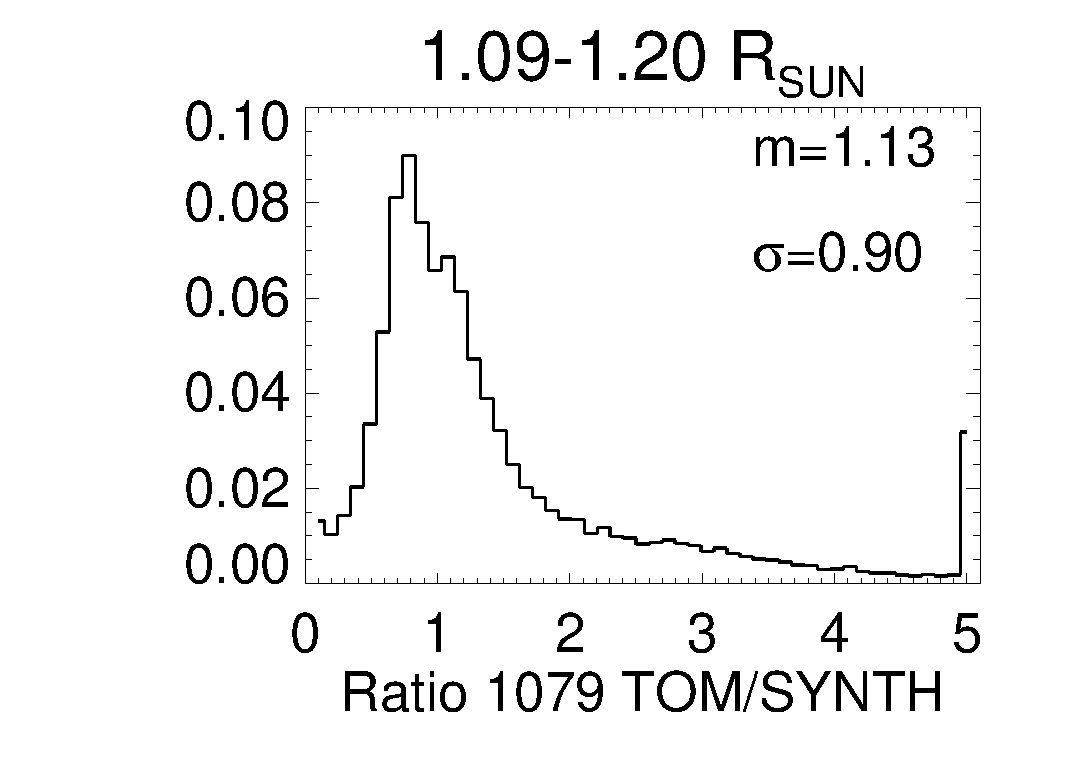
\includegraphics[height=0.2\textwidth,clip=]{fig/comparison_ucomp_Sept2022_tom_vs_synth_E1079_ratio_range1_090-1_200_Rsun.eps}
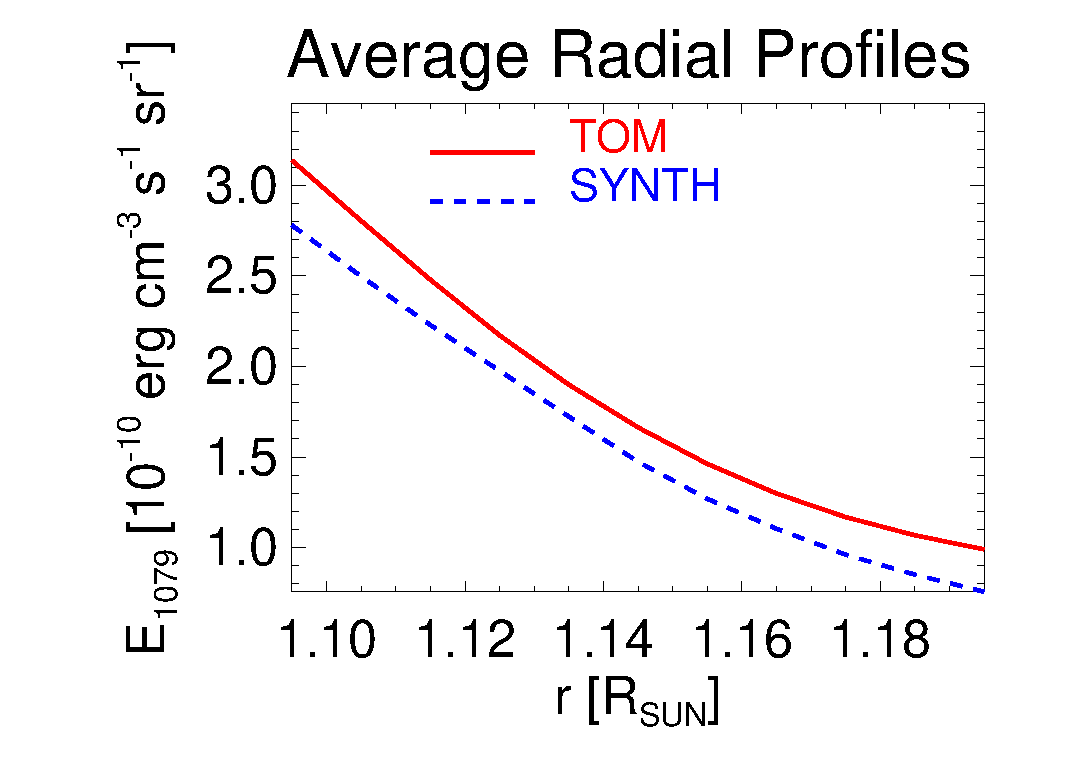
\includegraphics[height=0.2\textwidth,clip=]{fig/Average_Radial_Profiles_ucomp_Sept2022_tom_vs_synth_E1079.eps}
\end{center}
}
}


\frame{
\titulo{3D $\Ne$ with Three Diagnostics}
{\footnotesize\sf
\azul{
~~~~~~~UCoMP-SRT\hskip 2.2cm AIA-DEMT\hskip 2.3cm KCOR-SRT
}
\vspace{-0.1cm}
\begin{center}
\includegraphics[width=0.32\textwidth,clip=]{fig/Ne_ucomp_1_105_Rsun.jpg}
\includegraphics[width=0.32\textwidth,clip=]{fig/Ne_aia_1_105_Rsun.jpg}
\includegraphics[width=0.32\textwidth,clip=]{fig/Ne_kcor_1_105_Rsun.jpg}
\includegraphics[width=0.32\textwidth,clip=]{fig/Ne_ucomp_1_145_Rsun.jpg}
\includegraphics[width=0.32\textwidth,clip=]{fig/Ne_aia_1_145_Rsun.jpg}
\includegraphics[width=0.32\textwidth,clip=]{fig/Ne_kcor_1_145_Rsun.jpg}
\includegraphics[width=0.32\textwidth,clip=]{fig/Ne_ucomp_1_195_Rsun.jpg}
\includegraphics[width=0.32\textwidth,clip=]{fig/Ne_aia_1_195_Rsun.jpg}
\includegraphics[width=0.32\textwidth,clip=]{fig/Ne_kcor_1_195_Rsun.jpg}
\end{center}
}
}

\frame{
\titulo{Comparison of Reconstructed $\Ne$}
{\footnotesize\sf
\vspace{+0.2cm}
\ \hskip 2.25cm {\bf UCoMP versus AIA \hskip 2.5cm UCoMP versus KCOR}
\begin{center}
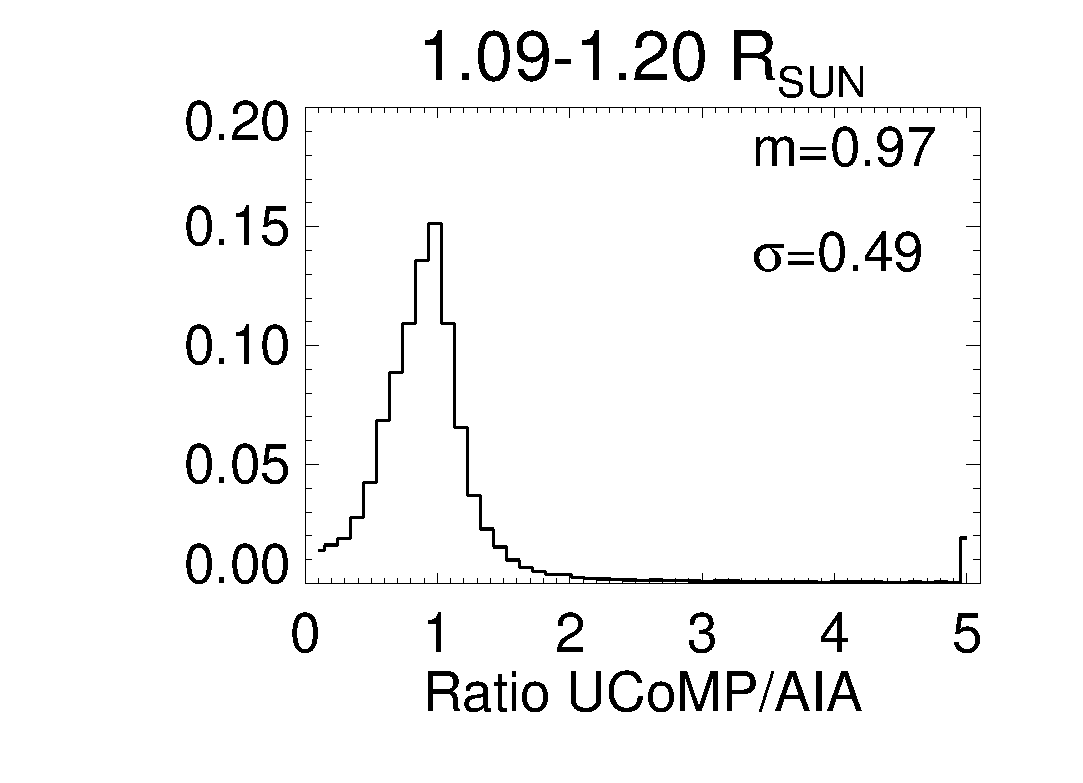
\includegraphics[width=0.45\textwidth,clip=]{fig/comparison_ucomp_vs_aia_ratio_range1_090-1_200_Rsun.eps}
\includegraphics[width=0.45\textwidth,clip=]{fig/comparison_kcor_vs_ucomp_ratio_range1_090-1_200_Rsun.eps}
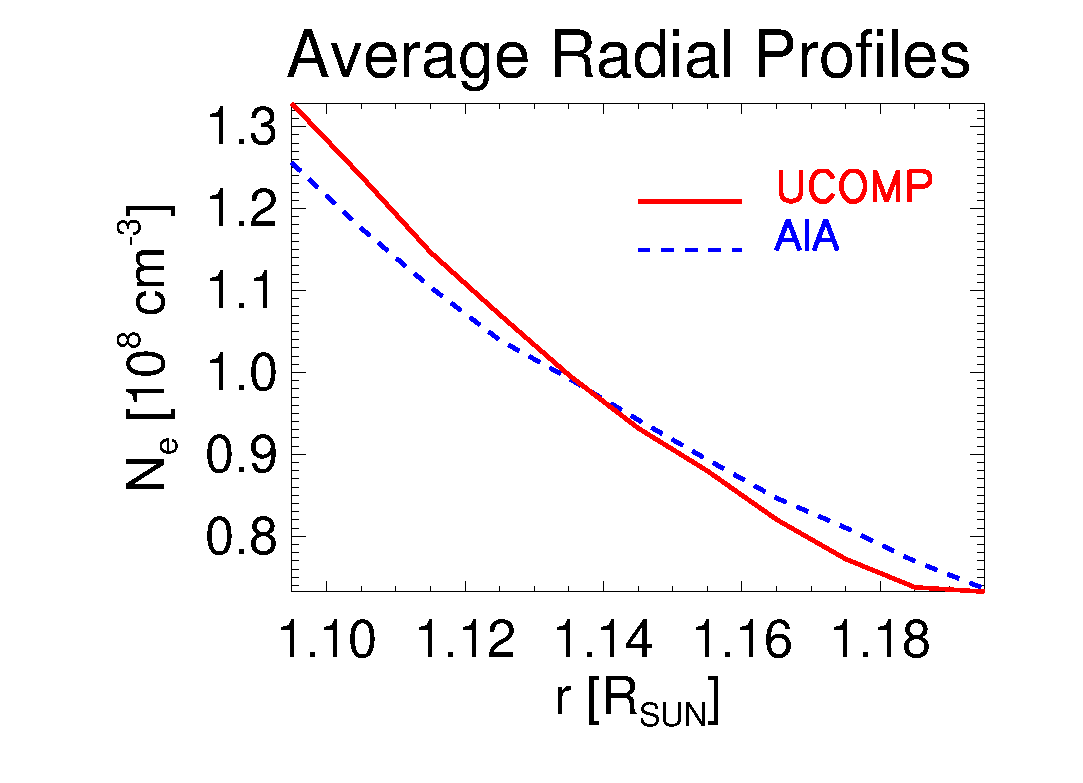
\includegraphics[width=0.45\textwidth,clip=]{fig/Average_Radial_Profiles_ucomp_vs_aia.eps}
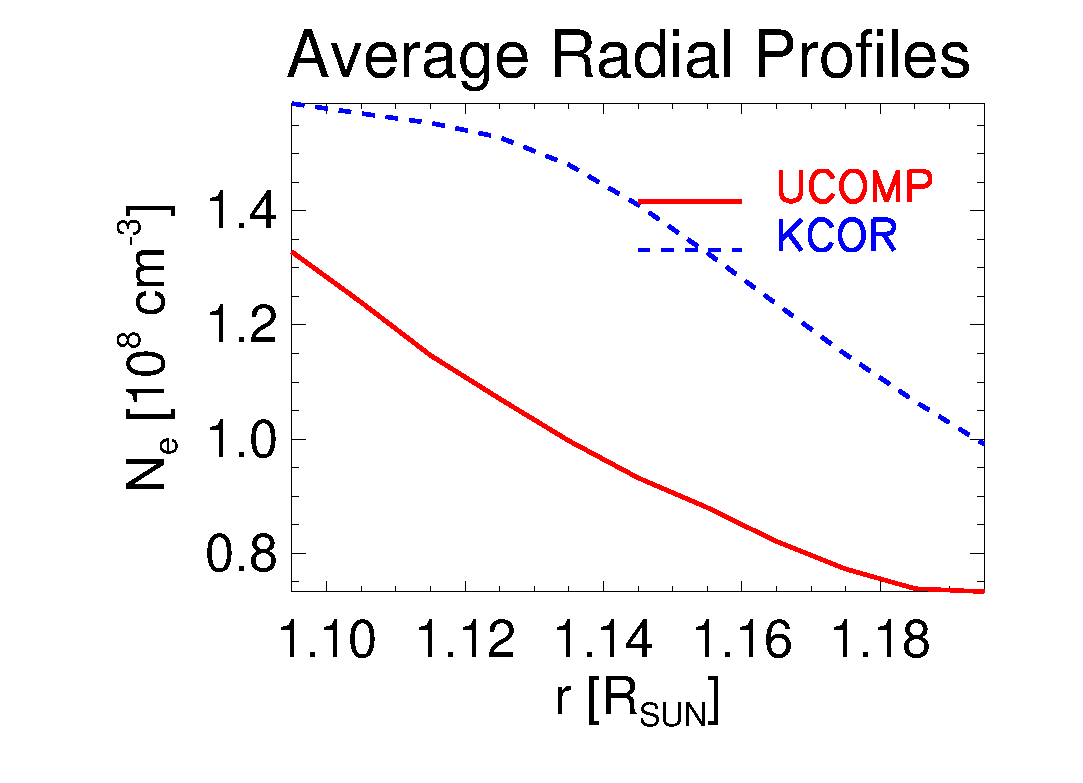
\includegraphics[width=0.45\textwidth,clip=]{fig/Average_Radial_Profiles_kcor_vs_ucomp.eps}
\end{center}
}
}


\end{document}



\title[Tomography: UCoMP versus AIA versus KCOR]
{\bf Tomography: UCoMP versus AIA versus KCOR}
\author[Vasquez \& Nuevo]
       {
       {\bf 
       Alberto M. Vasquez \& Federico A. Nuevo}
       \vskip 0.25cm
       {\bf 
\tiny
Instituto de Astronomía y Física del Espacio (IAFE), Buenos Aires--Argentina\\
       }
       }
\institute[]
{
\begin{center}
\framebox{\includegraphics[height=0.125\linewidth]{fig/logo_IAFE.eps}}
\vskip 3cm
{\bf March 2025}
\end{center}
}

\begin{document}


\frame{
\titulo{Tomography: UCoMP versus AIA versus KCOR}
{\tiny\sf
\begin{itemize}
\item \azul{Solar rotational tomography (SRT)} makes use of 1/2 solar rotation (14-day) long sequences of coronal images to determine the \azul{3D distribution of various physical quantities} of the corona, depending on the observed wavelength range.
\salto
\item Using \azul{WL pB} images (e.g. KCOR, C2, Metis), SRT allows determination of the \azul{3D $\Ne$}.
\salto
\item Using \azul{EUV} images with a given filter (e.g. AIA 171\,\AA), SRT allows determination of the \azul{3D band-emissivity}.\\ 
Based on the reconstructed band-emissivity for various filters independently (e.g. AIA 171, 193, and 211\,\AA),\\ 
a local-DEM analysis can be carried out at each location of the corona to determine the \azul{3D $\Ne$} and \azul{$\Te$}.\\ 
The combined procedure is known as DEM-Tomography, or \azul{DEMT}.
\salto
\item Using \azul{UCoMP} total-line (wavelength-integrated) images, SRT allows determination of the \azul{3D line emissivity}.
\salto 
\item For a specific period (September 2022), we carried out:
\saltito
a) \azul{UCoMP-SRT} with 1074 and 1079 nm images to determine their respective \azul{3D emissivity maps}.\\
\ \ \ \ The 1074:1079 emissivity-ratio can then be used to determine 3D $\Ne$.
\saltito
b) \azul{AIA-DEMT} (using filters 171, 193 and 211\,\AA) to determine the \azul{3D $\Ne$} and \azul{$\Te$},\\
\ \ \ \ in turn used with CHIANTI to compute \azul{3D synthetic emissivity maps} for the lines at 1074 and 1079 nm.
\saltito
c) \azul{KCOR-SRT} to determine the 3D distribution of $\Ne$.
\salto
\item These instruments allow reconstructions over a common range of heights $1.1-1.2\,\Rs$. We compare:
\saltito 
1) The tomographic UCoMP-SRT line emissivities against the synthetic prediction based on AIA-DEMT.
\saltito
2) {The 3D $\Ne$ derived from UCoMP-SRT, derived from AIA-DEMT, and derived from KCOR-SRT.}
\end{itemize}
}}

\frame{
\titulo{3D Coronal Emissivity at 1074 nm}
{\footnotesize\sf
\begin{center}
Lat/Lon maps of UCoMP 3D \azul{Tomographic} 1074-Emissivity\\
\includegraphics[width=0.32\textwidth,clip=]{fig/x_comp1074_1_105_Rsun.jpg}
\includegraphics[width=0.32\textwidth,clip=]{fig/x_comp1074_1_145_Rsun.jpg}
\includegraphics[width=0.32\textwidth,clip=]{fig/x_comp1074_1_195_Rsun.jpg}
\salto
Lat/Lon maps of AIA(171-193-211)-DEMT 3D \azul{Synthetic} 1074-Emissivity\\
\includegraphics[width=0.32\textwidth,clip=]{fig/x_comp1074_synth_1_105_Rsun.jpg}
\includegraphics[width=0.32\textwidth,clip=]{fig/x_comp1074_synth_1_145_Rsun.jpg}
\includegraphics[width=0.32\textwidth,clip=]{fig/x_comp1074_synth_1_195_Rsun.jpg}
\salto
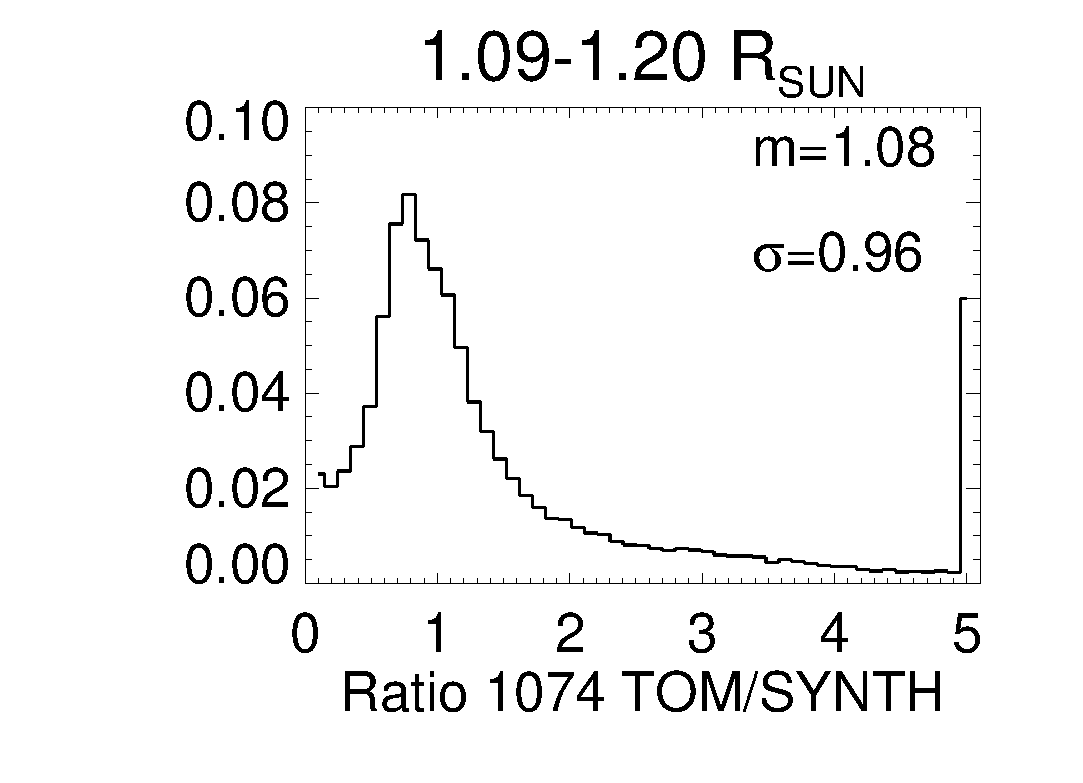
\includegraphics[height=0.2\textwidth,clip=]{fig/comparison_ucomp_Sept2022_tom_vs_synth_E1074_ratio_range1_090-1_200_Rsun.eps}
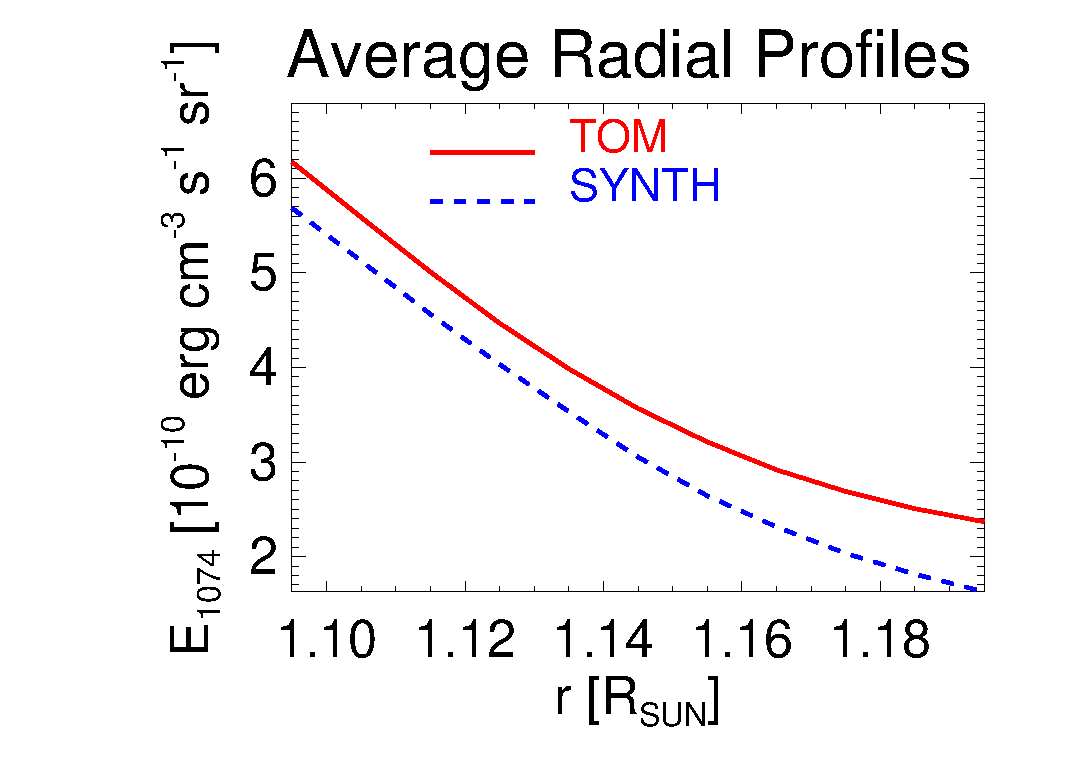
\includegraphics[height=0.2\textwidth,clip=]{fig/Average_Radial_Profiles_ucomp_Sept2022_tom_vs_synth_E1074.eps}
\end{center}
}
}

\frame{
\titulo{3D Coronal Emissivity at 1079 nm}
{\footnotesize\sf
\begin{center}
Lat/Lon maps of UCoMP 3D \azul{Tomographic} 1079-Emissivity\\
\includegraphics[width=0.32\textwidth,clip=]{fig/x_comp1079_1_105_Rsun.jpg}
\includegraphics[width=0.32\textwidth,clip=]{fig/x_comp1079_1_145_Rsun.jpg}
\includegraphics[width=0.32\textwidth,clip=]{fig/x_comp1079_1_195_Rsun.jpg}
\salto
Lat/Lon maps of AIA(171-193-211)-DEMT 3D \azul{Synthetic} 1079-Emissivity\\
\includegraphics[width=0.32\textwidth,clip=]{fig/x_comp1079_synth_1_105_Rsun.jpg}
\includegraphics[width=0.32\textwidth,clip=]{fig/x_comp1079_synth_1_145_Rsun.jpg}
\includegraphics[width=0.32\textwidth,clip=]{fig/x_comp1079_synth_1_195_Rsun.jpg}
\salto
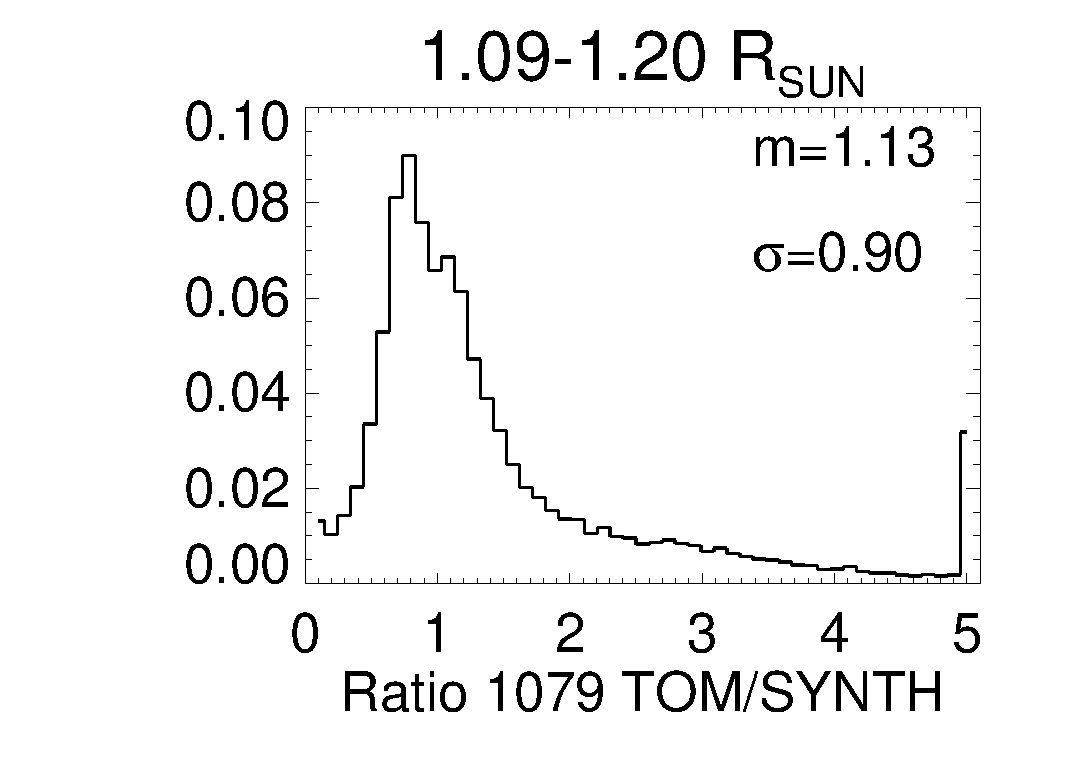
\includegraphics[height=0.2\textwidth,clip=]{fig/comparison_ucomp_Sept2022_tom_vs_synth_E1079_ratio_range1_090-1_200_Rsun.eps}
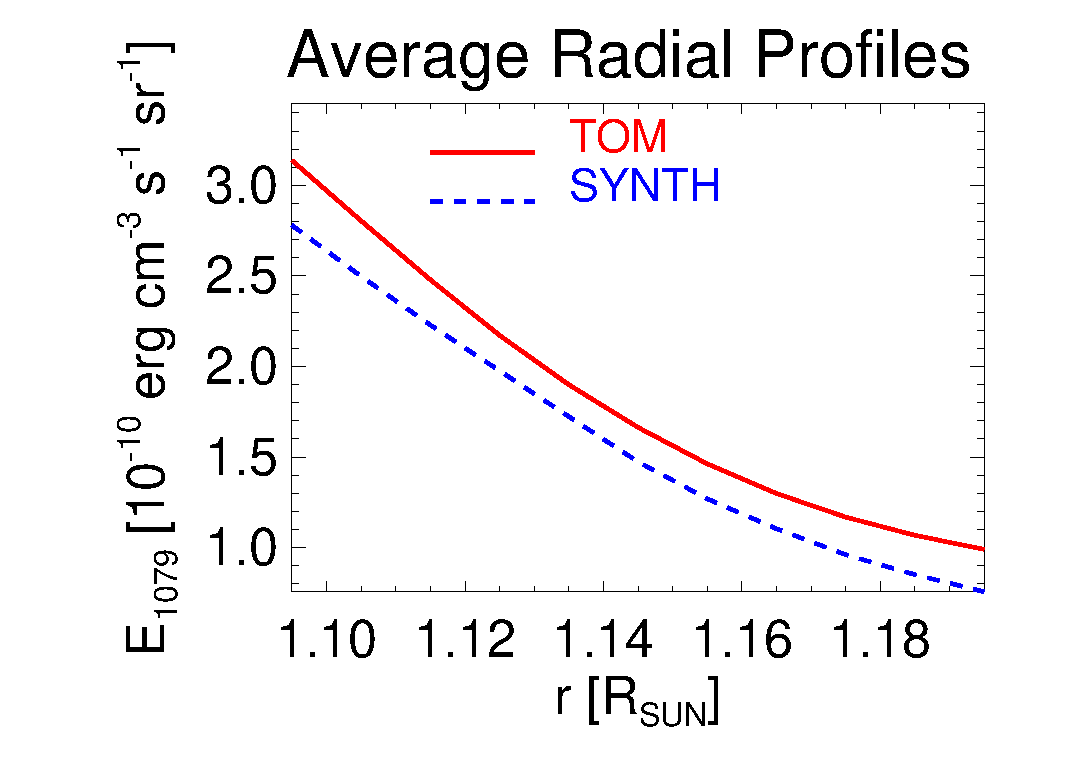
\includegraphics[height=0.2\textwidth,clip=]{fig/Average_Radial_Profiles_ucomp_Sept2022_tom_vs_synth_E1079.eps}
\end{center}
}
}


\frame{
\titulo{3D $\Ne$ with Three Diagnostics}
{\footnotesize\sf
\azul{
~~~~~~~UCoMP-SRT\hskip 2.2cm AIA-DEMT\hskip 2.3cm KCOR-SRT
}
\vspace{-0.1cm}
\begin{center}
\includegraphics[width=0.32\textwidth,clip=]{fig/Ne_ucomp_1_105_Rsun.jpg}
\includegraphics[width=0.32\textwidth,clip=]{fig/Ne_aia_1_105_Rsun.jpg}
\includegraphics[width=0.32\textwidth,clip=]{fig/Ne_kcor_1_105_Rsun.jpg}
\includegraphics[width=0.32\textwidth,clip=]{fig/Ne_ucomp_1_145_Rsun.jpg}
\includegraphics[width=0.32\textwidth,clip=]{fig/Ne_aia_1_145_Rsun.jpg}
\includegraphics[width=0.32\textwidth,clip=]{fig/Ne_kcor_1_145_Rsun.jpg}
\includegraphics[width=0.32\textwidth,clip=]{fig/Ne_ucomp_1_195_Rsun.jpg}
\includegraphics[width=0.32\textwidth,clip=]{fig/Ne_aia_1_195_Rsun.jpg}
\includegraphics[width=0.32\textwidth,clip=]{fig/Ne_kcor_1_195_Rsun.jpg}
\end{center}
}
}

\frame{
\titulo{Comparison of Reconstructed $\Ne$}
{\footnotesize\sf
\vspace{+0.2cm}
\ \hskip 2.25cm {\bf UCoMP versus AIA \hskip 2.5cm UCoMP versus KCOR}
\begin{center}
\includegraphics[width=0.45\textwidth,clip=]{fig/comparison_ucomp_vs_aia_ratio_range1_090-1_200_Rsun.eps}
\includegraphics[width=0.45\textwidth,clip=]{fig/comparison_kcor_vs_ucomp_ratio_range1_090-1_200_Rsun.eps}
\includegraphics[width=0.45\textwidth,clip=]{fig/Average_Radial_Profiles_ucomp_vs_aia.eps}
\includegraphics[width=0.45\textwidth,clip=]{fig/Average_Radial_Profiles_kcor_vs_ucomp.eps}
\end{center}
}
}


\end{document}



\title[Tomography: UCoMP versus AIA versus KCOR]
{\bf Tomography: UCoMP versus AIA versus KCOR}
\author[Vasquez \& Nuevo]
       {
       {\bf 
       Alberto M. Vasquez \& Federico A. Nuevo}
       \vskip 0.25cm
       {\bf 
\tiny
Instituto de Astronomía y Física del Espacio (IAFE), Buenos Aires--Argentina\\
       }
       }
\institute[]
{
\begin{center}
\framebox{\includegraphics[height=0.125\linewidth]{fig/logo_IAFE.eps}}
\vskip 3cm
{\bf March 2025}
\end{center}
}

\begin{document}


\frame{
\titulo{Tomography: UCoMP versus AIA versus KCOR}
{\tiny\sf
\begin{itemize}
\item \azul{Solar rotational tomography (SRT)} makes use of 1/2 solar rotation (14-day) long sequences of coronal images to determine the \azul{3D distribution of various physical quantities} of the corona, depending on the observed wavelength range.
\salto
\item Using \azul{WL pB} images (e.g. KCOR, C2, Metis), SRT allows determination of the \azul{3D $\Ne$}.
\salto
\item Using \azul{EUV} images with a given filter (e.g. AIA 171\,\AA), SRT allows determination of the \azul{3D band-emissivity}.\\ 
Based on the reconstructed band-emissivity for various filters independently (e.g. AIA 171, 193, and 211\,\AA),\\ 
a local-DEM analysis can be carried out at each location of the corona to determine the \azul{3D $\Ne$} and \azul{$\Te$}.\\ 
The combined procedure is known as DEM-Tomography, or \azul{DEMT}.
\salto
\item Using \azul{UCoMP} total-line (wavelength-integrated) images, SRT allows determination of the \azul{3D line emissivity}.
\salto 
\item For a specific period (September 2022), we carried out:
\saltito
a) \azul{UCoMP-SRT} with 1074 and 1079 nm images to determine their respective \azul{3D emissivity maps}.\\
\ \ \ \ The 1074:1079 emissivity-ratio can then be used to determine 3D $\Ne$.
\saltito
b) \azul{AIA-DEMT} (using filters 171, 193 and 211\,\AA) to determine the \azul{3D $\Ne$} and \azul{$\Te$},\\
\ \ \ \ in turn used with CHIANTI to compute \azul{3D synthetic emissivity maps} for the lines at 1074 and 1079 nm.
\saltito
c) \azul{KCOR-SRT} to determine the 3D distribution of $\Ne$.
\salto
\item These instruments allow reconstructions over a common range of heights $1.1-1.2\,\Rs$. We compare:
\saltito 
1) The tomographic UCoMP-SRT line emissivities against the synthetic prediction based on AIA-DEMT.
\saltito
2) {The 3D $\Ne$ derived from UCoMP-SRT, derived from AIA-DEMT, and derived from KCOR-SRT.}
\end{itemize}
}}

\frame{
\titulo{3D Coronal Emissivity at 1074 nm}
{\footnotesize\sf
\begin{center}
Lat/Lon maps of UCoMP 3D \azul{Tomographic} 1074-Emissivity\\
\includegraphics[width=0.32\textwidth,clip=]{fig/x_comp1074_1_105_Rsun.jpg}
\includegraphics[width=0.32\textwidth,clip=]{fig/x_comp1074_1_145_Rsun.jpg}
\includegraphics[width=0.32\textwidth,clip=]{fig/x_comp1074_1_195_Rsun.jpg}
\salto
Lat/Lon maps of AIA(171-193-211)-DEMT 3D \azul{Synthetic} 1074-Emissivity\\
\includegraphics[width=0.32\textwidth,clip=]{fig/x_comp1074_synth_1_105_Rsun.jpg}
\includegraphics[width=0.32\textwidth,clip=]{fig/x_comp1074_synth_1_145_Rsun.jpg}
\includegraphics[width=0.32\textwidth,clip=]{fig/x_comp1074_synth_1_195_Rsun.jpg}
\salto
\includegraphics[height=0.2\textwidth,clip=]{fig/comparison_ucomp_Sept2022_tom_vs_synth_E1074_ratio_range1_090-1_200_Rsun.eps}
\includegraphics[height=0.2\textwidth,clip=]{fig/Average_Radial_Profiles_ucomp_Sept2022_tom_vs_synth_E1074.eps}
\end{center}
}
}

\frame{
\titulo{3D Coronal Emissivity at 1079 nm}
{\footnotesize\sf
\begin{center}
Lat/Lon maps of UCoMP 3D \azul{Tomographic} 1079-Emissivity\\
\includegraphics[width=0.32\textwidth,clip=]{fig/x_comp1079_1_105_Rsun.jpg}
\includegraphics[width=0.32\textwidth,clip=]{fig/x_comp1079_1_145_Rsun.jpg}
\includegraphics[width=0.32\textwidth,clip=]{fig/x_comp1079_1_195_Rsun.jpg}
\salto
Lat/Lon maps of AIA(171-193-211)-DEMT 3D \azul{Synthetic} 1079-Emissivity\\
\includegraphics[width=0.32\textwidth,clip=]{fig/x_comp1079_synth_1_105_Rsun.jpg}
\includegraphics[width=0.32\textwidth,clip=]{fig/x_comp1079_synth_1_145_Rsun.jpg}
\includegraphics[width=0.32\textwidth,clip=]{fig/x_comp1079_synth_1_195_Rsun.jpg}
\salto
\includegraphics[height=0.2\textwidth,clip=]{fig/comparison_ucomp_Sept2022_tom_vs_synth_E1079_ratio_range1_090-1_200_Rsun.eps}
\includegraphics[height=0.2\textwidth,clip=]{fig/Average_Radial_Profiles_ucomp_Sept2022_tom_vs_synth_E1079.eps}
\end{center}
}
}


\frame{
\titulo{3D $\Ne$ with Three Diagnostics}
{\footnotesize\sf
\azul{
~~~~~~~UCoMP-SRT\hskip 2.2cm AIA-DEMT\hskip 2.3cm KCOR-SRT
}
\vspace{-0.1cm}
\begin{center}
\includegraphics[width=0.32\textwidth,clip=]{fig/Ne_ucomp_1_105_Rsun.jpg}
\includegraphics[width=0.32\textwidth,clip=]{fig/Ne_aia_1_105_Rsun.jpg}
\includegraphics[width=0.32\textwidth,clip=]{fig/Ne_kcor_1_105_Rsun.jpg}
\includegraphics[width=0.32\textwidth,clip=]{fig/Ne_ucomp_1_145_Rsun.jpg}
\includegraphics[width=0.32\textwidth,clip=]{fig/Ne_aia_1_145_Rsun.jpg}
\includegraphics[width=0.32\textwidth,clip=]{fig/Ne_kcor_1_145_Rsun.jpg}
\includegraphics[width=0.32\textwidth,clip=]{fig/Ne_ucomp_1_195_Rsun.jpg}
\includegraphics[width=0.32\textwidth,clip=]{fig/Ne_aia_1_195_Rsun.jpg}
\includegraphics[width=0.32\textwidth,clip=]{fig/Ne_kcor_1_195_Rsun.jpg}
\end{center}
}
}

\frame{
\titulo{Comparison of Reconstructed $\Ne$}
{\footnotesize\sf
\vspace{+0.2cm}
\ \hskip 2.25cm {\bf UCoMP versus AIA \hskip 2.5cm UCoMP versus KCOR}
\begin{center}
\includegraphics[width=0.45\textwidth,clip=]{fig/comparison_ucomp_vs_aia_ratio_range1_090-1_200_Rsun.eps}
\includegraphics[width=0.45\textwidth,clip=]{fig/comparison_kcor_vs_ucomp_ratio_range1_090-1_200_Rsun.eps}
\includegraphics[width=0.45\textwidth,clip=]{fig/Average_Radial_Profiles_ucomp_vs_aia.eps}
\includegraphics[width=0.45\textwidth,clip=]{fig/Average_Radial_Profiles_kcor_vs_ucomp.eps}
\end{center}
}
}


\end{document}



\title[Tomography: UCoMP versus AIA versus KCOR]
{\bf Tomography: UCoMP versus AIA versus KCOR}
\author[Vasquez \& Nuevo]
       {
       {\bf 
       Alberto M. Vasquez \& Federico A. Nuevo}
       \vskip 0.25cm
       {\bf 
\tiny
Instituto de Astronomía y Física del Espacio (IAFE), Buenos Aires--Argentina\\
       }
       }
\institute[]
{
\begin{center}
\framebox{\includegraphics[height=0.125\linewidth]{fig/logo_IAFE.eps}}
\vskip 3cm
{\bf March 2025}
\end{center}
}

\begin{document}


\frame{
\titulo{Tomography: UCoMP versus AIA versus KCOR}
{\tiny\sf
\begin{itemize}
\item \azul{Solar rotational tomography (SRT)} makes use of 1/2 solar rotation (14-day) long sequences of coronal images to determine the \azul{3D distribution of various physical quantities} of the corona, depending on the observed wavelength range.
\salto
\item Using \azul{WL pB} images (e.g. KCOR, C2, Metis), SRT allows determination of the \azul{3D $\Ne$}.
\salto
\item Using \azul{EUV} images with a given filter (e.g. AIA 171\,\AA), SRT allows determination of the \azul{3D band-emissivity}.\\ 
Based on the reconstructed band-emissivity for various filters independently (e.g. AIA 171, 193, and 211\,\AA),\\ 
a local-DEM analysis can be carried out at each location of the corona to determine the \azul{3D $\Ne$} and \azul{$\Te$}.\\ 
The combined procedure is known as DEM-Tomography, or \azul{DEMT}.
\salto
\item Using \azul{UCoMP} total-line (wavelength-integrated) images, SRT allows determination of the \azul{3D line emissivity}.
\salto 
\item For a specific period (September 2022), we carried out:
\saltito
a) \azul{UCoMP-SRT} with 1074 and 1079 nm images to determine their respective \azul{3D emissivity maps}.\\
\ \ \ \ The 1074:1079 emissivity-ratio can then be used to determine 3D $\Ne$.
\saltito
b) \azul{AIA-DEMT} (using filters 171, 193 and 211\,\AA) to determine the \azul{3D $\Ne$} and \azul{$\Te$},\\
\ \ \ \ in turn used with CHIANTI to compute \azul{3D synthetic emissivity maps} for the lines at 1074 and 1079 nm.
\saltito
c) \azul{KCOR-SRT} to determine the 3D distribution of $\Ne$.
\salto
\item These instruments allow reconstructions over a common range of heights $1.1-1.2\,\Rs$. We compare:
\saltito 
1) The tomographic UCoMP-SRT line emissivities against the synthetic prediction based on AIA-DEMT.
\saltito
2) {The 3D $\Ne$ derived from UCoMP-SRT, derived from AIA-DEMT, and derived from KCOR-SRT.}
\end{itemize}
}}

\frame{
\titulo{3D Coronal Emissivity at 1074 nm}
{\footnotesize\sf
\begin{center}
Lat/Lon maps of UCoMP 3D \azul{Tomographic} 1074-Emissivity\\
\includegraphics[width=0.32\textwidth,clip=]{fig/x_comp1074_1_105_Rsun.jpg}
\includegraphics[width=0.32\textwidth,clip=]{fig/x_comp1074_1_145_Rsun.jpg}
\includegraphics[width=0.32\textwidth,clip=]{fig/x_comp1074_1_195_Rsun.jpg}
\salto
Lat/Lon maps of AIA(171-193-211)-DEMT 3D \azul{Synthetic} 1074-Emissivity\\
\includegraphics[width=0.32\textwidth,clip=]{fig/x_comp1074_synth_1_105_Rsun.jpg}
\includegraphics[width=0.32\textwidth,clip=]{fig/x_comp1074_synth_1_145_Rsun.jpg}
\includegraphics[width=0.32\textwidth,clip=]{fig/x_comp1074_synth_1_195_Rsun.jpg}
\salto
\includegraphics[height=0.2\textwidth,clip=]{fig/comparison_ucomp_Sept2022_tom_vs_synth_E1074_ratio_range1_090-1_200_Rsun.eps}
\includegraphics[height=0.2\textwidth,clip=]{fig/Average_Radial_Profiles_ucomp_Sept2022_tom_vs_synth_E1074.eps}
\end{center}
}
}

\frame{
\titulo{3D Coronal Emissivity at 1079 nm}
{\footnotesize\sf
\begin{center}
Lat/Lon maps of UCoMP 3D \azul{Tomographic} 1079-Emissivity\\
\includegraphics[width=0.32\textwidth,clip=]{fig/x_comp1079_1_105_Rsun.jpg}
\includegraphics[width=0.32\textwidth,clip=]{fig/x_comp1079_1_145_Rsun.jpg}
\includegraphics[width=0.32\textwidth,clip=]{fig/x_comp1079_1_195_Rsun.jpg}
\salto
Lat/Lon maps of AIA(171-193-211)-DEMT 3D \azul{Synthetic} 1079-Emissivity\\
\includegraphics[width=0.32\textwidth,clip=]{fig/x_comp1079_synth_1_105_Rsun.jpg}
\includegraphics[width=0.32\textwidth,clip=]{fig/x_comp1079_synth_1_145_Rsun.jpg}
\includegraphics[width=0.32\textwidth,clip=]{fig/x_comp1079_synth_1_195_Rsun.jpg}
\salto
\includegraphics[height=0.2\textwidth,clip=]{fig/comparison_ucomp_Sept2022_tom_vs_synth_E1079_ratio_range1_090-1_200_Rsun.eps}
\includegraphics[height=0.2\textwidth,clip=]{fig/Average_Radial_Profiles_ucomp_Sept2022_tom_vs_synth_E1079.eps}
\end{center}
}
}


\frame{
\titulo{3D $\Ne$ with Three Diagnostics}
{\footnotesize\sf
\azul{
~~~~~~~UCoMP-SRT\hskip 2.2cm AIA-DEMT\hskip 2.3cm KCOR-SRT
}
\vspace{-0.1cm}
\begin{center}
\includegraphics[width=0.32\textwidth,clip=]{fig/Ne_ucomp_1_105_Rsun.jpg}
\includegraphics[width=0.32\textwidth,clip=]{fig/Ne_aia_1_105_Rsun.jpg}
\includegraphics[width=0.32\textwidth,clip=]{fig/Ne_kcor_1_105_Rsun.jpg}
\includegraphics[width=0.32\textwidth,clip=]{fig/Ne_ucomp_1_145_Rsun.jpg}
\includegraphics[width=0.32\textwidth,clip=]{fig/Ne_aia_1_145_Rsun.jpg}
\includegraphics[width=0.32\textwidth,clip=]{fig/Ne_kcor_1_145_Rsun.jpg}
\includegraphics[width=0.32\textwidth,clip=]{fig/Ne_ucomp_1_195_Rsun.jpg}
\includegraphics[width=0.32\textwidth,clip=]{fig/Ne_aia_1_195_Rsun.jpg}
\includegraphics[width=0.32\textwidth,clip=]{fig/Ne_kcor_1_195_Rsun.jpg}
\end{center}
}
}

\frame{
\titulo{Comparison of Reconstructed $\Ne$}
{\footnotesize\sf
\vspace{+0.2cm}
\ \hskip 2.25cm {\bf UCoMP versus AIA \hskip 2.5cm UCoMP versus KCOR}
\begin{center}
\includegraphics[width=0.45\textwidth,clip=]{fig/comparison_ucomp_vs_aia_ratio_range1_090-1_200_Rsun.eps}
\includegraphics[width=0.45\textwidth,clip=]{fig/comparison_kcor_vs_ucomp_ratio_range1_090-1_200_Rsun.eps}
\includegraphics[width=0.45\textwidth,clip=]{fig/Average_Radial_Profiles_ucomp_vs_aia.eps}
\includegraphics[width=0.45\textwidth,clip=]{fig/Average_Radial_Profiles_kcor_vs_ucomp.eps}
\end{center}
}
}


\end{document}

